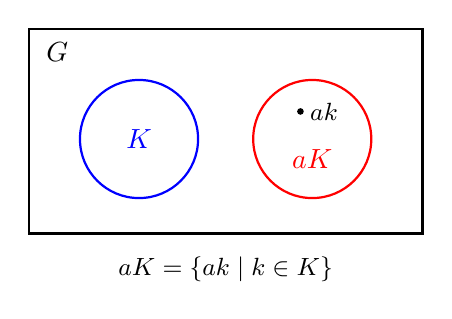
\begin{tikzpicture}[scale=1]
  \draw[thick] (0,0) rectangle (5,2.6);
  \node[anchor=north west] at (0.1,2.55) {$G$};
  \draw[thick, blue] (1.4,1.2) circle (0.75);
  \node[blue] at (1.4,1.2) {$K$};
  \draw[thick, red] (3.6,1.2) circle (0.75);
  \node[red] at (3.6,0.95) {$aK$};
  \fill (3.45,1.55) circle (1.2pt) node[right, font=\small] {$ak$};
  \node[font=\small, align=center] at (2.5,-0.45) {$aK=\{ak \mid k\in K\}$};
\end{tikzpicture}
